%----------------------------------------------------------------------------
\chapter{Automatic license plate recognition}

Automatic license plate recognition (ALPR) refers to a technology that identifies vehicles based on their number plates. It is based on Optical character recognition. Traditionally, these systems are used to find stolen vehicles, check for road usage permits, measure vehicle speed, or operate parking garages. The technology is also suitable for tracking vehicles and collecting location data. This may be to the benefit of the authorities, but in Europe, it raises privacy concerns, as drivers have the right to data privacy.

ALPR systems can be categorized according to several aspects. There are fixed (pre-installed) and mobile (cameras in vehicles) systems based on their mobility. According to another aspect, some systems perform on-device image evaluation, while others process them remotely (like on a central computer or a server farm). The variants are illustrated in Figure \ref{fig:alpr-systems}. Both solutions have pros and contras in terms of network bandwidth- and hardware requirements.

\begin{figure}[htb]
 \centerline{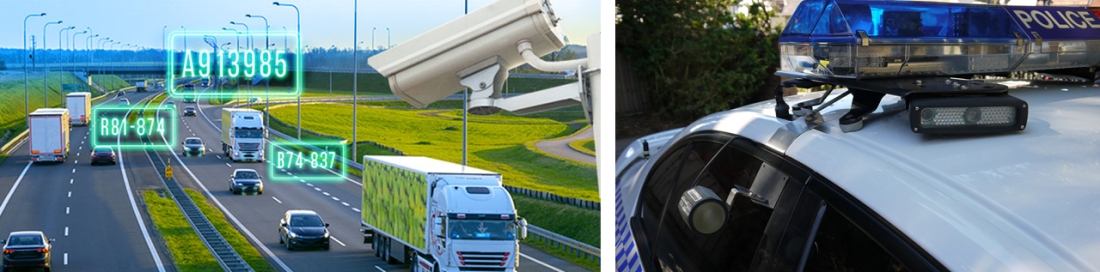
\includegraphics[width=1.0\columnwidth]{.//Figure/ALPR/alpr-systems.png}}
 \caption{Pre-installed closed-circuit ALPR system\cite{ImageFixedALPR} (left) and a police car equipped with mobile ALPR\cite{ImageMobileALPR} (right).}
 \label{fig:alpr-systems}
\end{figure}

\section{History}

The technology began to spread worldwide in the 2000s; however, the first ALPR systems were in service as early as the late 1970s. The first system was created in 1976 in the UK by the Police Scientific Development Branch. Their solution has been installed to monitor the A1 road's traffic and to look for stolen vehicles. The first arrest based on ALPR identification of a stolen car happened in 1981\cite{ANPR_history}.

As the technology evolved, more sophisticated solutions emerged. Fixed cameras began to form coherent networks, and thanks to hardware developments, previously expensive and cumbersome systems became affordable and widely available. The proliferation of the systems was further facilitated by changing license plates in many countries (like in the Netherlands) to help ALPR operation\cite{DutchLicensePlates}.

During the 1990s, mobile ALPR systems also appeared. This was due to the elimination of special hardware requirements, and the more robust solutions no longer required certain view angles or conditions to work. A challenging task, in this case, is solving the power supply requirements of the hardware from a battery. Providing an internet connection while moving is also a requirement. These have been challenging issues in the past; nowadays, they are no longer limiting factors.

\section{Components}

There are many versions of ALPR solutions that regularly differ from each other. Still, below I try to give a general picture of what image processing tasks arise in an ALPR system\cite{ANPR} (without claiming completeness):

\begin{itemize}
\item Plate localization is the process of finding and isolating the license plates. This can be either done with object detection or semantic segmentation.
\item Plate resizing and orientation try to minimize the skew of an image and adjust the dimensions to the required size. Various heuristics (like Projection Profile Method\cite{ProjectionProfileMethod}) exist to determine skew and apply projection afterward. A recent solution is the use of attention-based transformer neural networks\cite{SpatialTransformerNetworks}.
\item Image manipulation is a collective concept for pixel-level transformations based on its statistical properties in the present work's context. The process can either be normalization (rescale values into a range of [0, 1]), standardization (rescale values to have 0 mean and a standard deviation of 1), grayscale conversion, a combination of these, or other. Care must be taken with these operations because the image quality significantly affects the effectiveness of subsequent steps.
\item Optical character recognition consists of character segmentation and classification - more about this in the OCR chapter.
\item Syntactic inspection is the process where country-specific information is taken into consideration (position of specific characters, length of the recognized sequence). The goal here is to extract and validate the correct identifier.
\item Averaging multiple images can significantly improve performance. It helps by averaging unwanted protruding effects, such as blur or reflection, that often occur in pictures of moving vehicles.
\end{itemize}

Not all ALPR systems explicitly separate the above points (for example, the OCR character segmentation- and classification can be done at once or as separate steps). These factors influence the usability of a solution - the key is the implementation and coordination of them.

\section{Challenges}

In the case of an ALPR system, there are numerous difficulties for which there are different solutions.

The variance of the images is quite large. Accurate operation at different times (day or night) and weather conditions (sunny, snowy, foggy, rainy) is also expected in most cases. Image manipulation techniques can overcome this problem to some extent. Devices can see the license plates in different sizes and angles depending on their installation. This is where plate localization, then proper resizing and orientation can help - although this cannot provide a solution for too distant, low-quality license plate images. Blurring caused by the movement of cars is also a problem. The answer to this is to use short-shutter cameras (~1/1000 second) with a global shutter. The effect of different shutter speeds are illustrated by Figure \ref{fig:shutter-speed}. Modern smartphones are generally capable of the required shutter speeds. However, the presence of the rolling shutter can still be an issue.

\begin{figure}[htb]
 \centerline{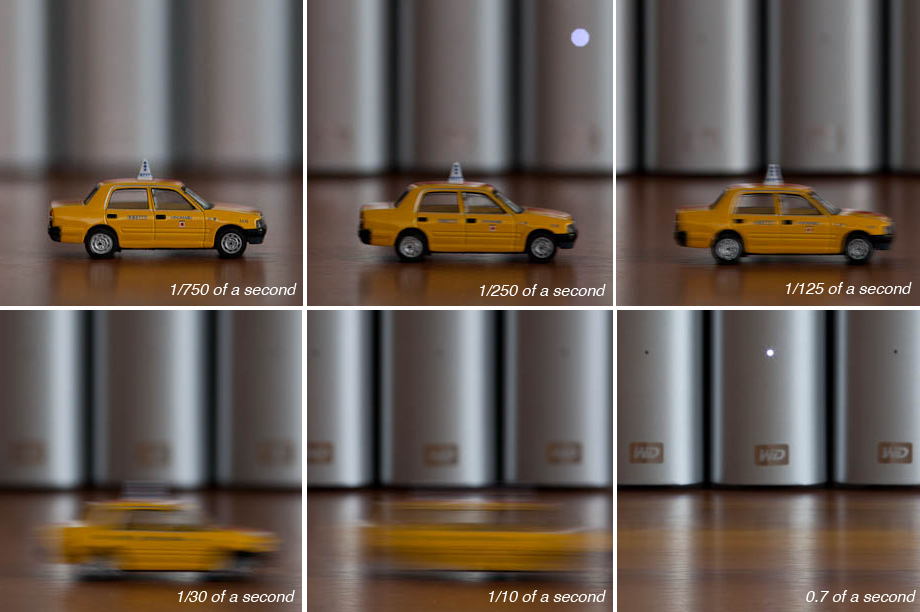
\includegraphics[width=1.0\columnwidth]{.//Figure/ALPR/shutter-speed.png}}
 \caption{The effect of shutter speed illustrated by a model car\cite{ShutterEffect}.}
 \label{fig:shutter-speed}
\end{figure}

Another common difficulty is the variety of number plates. License plates can have various structures, colors, and fonts, and their shape can also vary. It is typical for single and multi-row license plates to be used within a country. For these reasons, most of the current ALPR systems can only be used satisfactorily in a given country. However, the situation in Europe has improved in recent years with the proliferation of EU number plates. Although ALPR processability is now considered in the design of most license plates, in some countries, few characters have almost the same symbol (like 0 and O in England). Outside of Europe, characters outside the Latin alphabet may also appear. Character variability is discussed in more detail in the OCR chapter. Dirt may also be present on license plates, or other objects may obscure their text. Deliberate circumvention attempts can be an additional difficulty for ALPR systems. This can be, for example, covering certain characters or using a surface that impairs visibility. I do not address this issue in this work.
\newpage

\section{Evaluation}

Most ALPR system publishers provide rough metrics about their solutions, making it difficult to compare them. I found two de-facto benchmark datasets for license plate identification. The first is the SSIG SegPlate Database\cite{SSIG-ALPR}, with 101 on-track vehicles captured by a static camera. The other is the UFPR-ALPR Dataset\cite{UFPR-ALPR}, containing 4,500 images with 30,000 number plate characters.

\begin{figure}[htb]
 \centerline{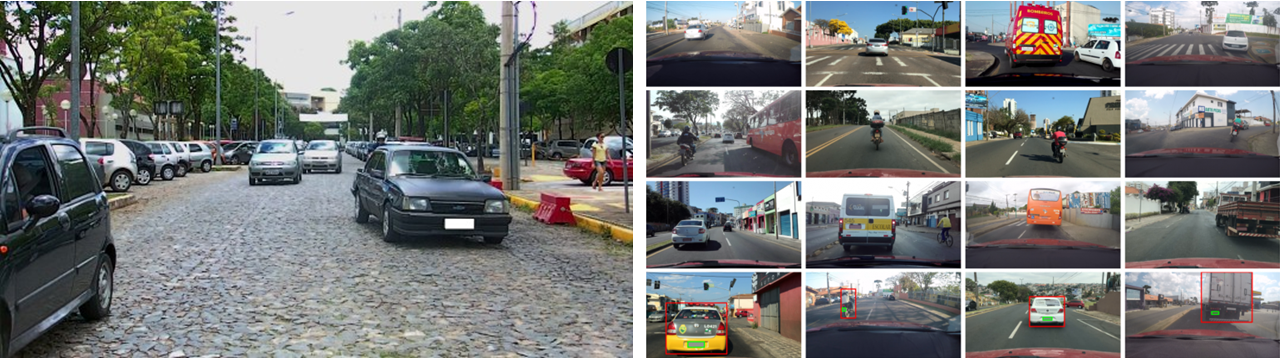
\includegraphics[width=1.0\columnwidth]{.//Figure/ALPR/alpr-datasets.png}}
 \caption{Samples from the SSIG SegPlate\cite{SSIG-ALPR} (left) and the UFPR-ALPR\cite{UFPR-ALPR} (right) datasets.}
 \label{fig:alpr-datasets}
\end{figure}

Sighthound\cite{Sighthound} and OpenALPR\cite{OpenALPR} are considered to be widespread market players. These solutions have been compared to a YOLO-based ALPR system by Laroca et al.\cite{RobustRealTimeALPR_YOLO}. Based on their performances on the SSIG dataset, Sighthound had 89.80\%, OpenALPR 93.03\%, and YOLO-ALPR 93.53\% accuracy. On the more challenging UFPR-ALPR dataset, Sighthound scored 47.39\%, OpenALPR 50.94\%, and YOLO-ALPR 64.89\% validation accuracy.

